\chapter{Praktische Umsetzung}

\section{Gehäuse}
\label{sec:org97effa6}
Das Gehäuse muss so dimensioniert sein, dass es Eurorack-kompatible Module beherbergen kann. Wichtig ist dabei vor allem der vertikale Abstand der Schienen, auf welchen die Module befestigt werden. Dieser misst laut dem \emph{Doepfer System A100 Handbuch Seite 3} ({Doepfer Musikelektronik Gmbh}, 2001) 3 HE (Höheneinheiten). 1 HE beträgt dabei \SI{44.45}{\milli\meter}. Die Breite der Module beträgt ein Vielfaches von \SI{5.08}{\milli\meter}, beziehungsweise 0.2 Zoll. Manche Gehäuse, wie beispielsweise die von der Firma Intellijel hergestellten, können auch Module, welche nur eine Höheneinheit hoch sind, beherbergen.

\section{Spannungsquelle}
\label{sec:org2dfb32d}
Eurorack Synthesizer arbeiten mit Spannungen von \SI{24}{\volt} peak to peak, benötigen also eine Spannungsquelle, welche \SI{-12}{\volt} bis \SI{+12}{\volt} bereitstellen kann. Manche Module benötigen außerdem eine separate \SI{5}{\volt} Leitung, um zum Beispiel Microcontroller zu betreiben. Eine beliebte Wahl in der DIY-Szene ist die Mean Well RT65B PSU, da sie \SI{\pm 12}{\volt} und \SI{5}{\volt} mit einer genügenden maximalen Stromstärke/Leistung bereitstellt, um ein Anfängersystem zu versorgen und verhältnismäßig günstig ist.

\section{Spannungsverteilung}
\label{sec:orgb739dbb}
Die Module werden über ein 10 Pin IDC-Flachbandkabel mit Strom versorgt. Dabei sind die mittleren 6 Pins durchverbunden und geerdet. Die äußeren vier Pins sind paarweise verbunden und liefern jeweils \SI{+12}{\volt} und \SI{-12}{\volt}. Der PIN, welcher auf \SI{-12}{\volt} liegt, ist üblicherweise rot gekennzeichnet.

\section{Transistoren abgleichen}
\label{sec:orgc591e71}
Manchmal werden Transistoren benötigt, welche einen möglichst gleichen internen Verstärkungsfaktor besitzen. Bereits aufeinander abgestimmte Transistorpaare sind zwar im Handel erhältlich, jedoch ist es einfach, das Abgleichen von Transistoren selbst vorzunehmen. Baut man den zu messenden Transistor in den folgenden Schaltkreis ein und legt man bei \(V_{CC}\) eine Spannung an, kann man seinen internen Verstärkungsfaktor herausfinden, indem man das Potential zwischen Punkt A (beim Kollektor des Transistors) und der Masse misst:

\begin{circuitikz}[european]
\draw{
(0,0) -- ++(3,0) node[ground]{}
(0,0) to[R, l=\SI{22}{\kilo\ohm}] ++(0,2.5) coordinate (T) to[R, l=\SI{220}{\kilo\ohm}] ++(0,2.5) -- ++(3,0) node[vcc]{$V_{CC}$} coordinate (U)
(T) -- ++(2,0) node[npn, tr circle](Q){}
(Q.C) to[R, l_=\SI{10}{\kilo\ohm}] (Q.C|-U)
(Q.E) to[R, l=\SI{1}{\kilo\ohm}] (Q.E|-0,0)
(Q.C) node[right] {A}
};
\end{circuitikz}

Diese Transistorenpaare sollten auf der Platine in unmittelbarer Nähe zueinander sein, da die Temperatur einen Einfluss auf die Eigenschaften eines Transistors hat.

\section{Vactrols}
\label{sec:orgfba15db}
Ein Vactrol, auf Deutsch oft Optokoppler, ist ein simpler, jedoch etwas ungenauer, spannungskontrollierbarer Widerstand, welcher aus einer Leuchtdiode und einem lichtempfindlichen Widerstand \ac{LDR} besteht. Er kann benutzt werden, um als variable Widerstände geschaltene Potentiometer zu ersetzen, um den zugehörigen Parameter spannungskontrollierbar zu machen. Der am Vactrol entstehende Widerstand ist näherungsweise invers proportional zur angelegten Spannung.

Während bereits gefertigte Vactrols im Handel erhältlich sind, ist es, vor allem in DIY Kreisen, üblich, sie selbst herzustellen. Dabei wird eine \ac{LED}, gemeinsam mit einem \ac{LDR} auf eine Art und Weise in ein lichtundurchlässiges Gehäuse (beispielsweise ein Schrumpfschlauch) gebaut, dass der \ac{LDR} von der \ac{LED} beleuchtet wird. 

\section{Module}
\label{sec:orgb554efa}

Im Folgenden werden die Module, welche den Synthesizer ausmachen, beschrieben. Jedes dieser Module besteht aus einem Panel, welches als User Interface dient und einer Platine, welche mit den elektronischen Komponenten bestückt ist. Panels besitzen mindestens eine Audiobuchse um \ac{CV}, Audio, Triggersignale und andere Arten von Spannungssignalen auszugeben, eine beliebige Anzahl an Audioeingängen für Kontrollspannungen, Audio-Inputs und ähnlichem und weitere Interfacekomponenten wie Beispielsweise Potentiometer, Schalter, Knöpfe und \acp{LED}.

Die elektronischen Komponenten können durch verschiedene Methoden zusammengeschalten werden, Beispiele dafür sind:
\begin{itemize}
\item Breadboards:
vor allem geeignet zum Erstellen von Prototypen
\item \ac{THT} Platinen:
eine schnelle Methode, um eine einzelne Platine zu fertigen
\item Selbst geätzte oder vorgefertigte Platinen:
eine Methode mit relativ geringem Fehlerpotential, ideal wenn eine größere Anzahl gleichartiger Platinen gefertigt werden sollen, beispielsweise für DIY-Kits
\item "`Deadbug"' Methode:
Eletronische Komponenten werden ohne Platine "`point to point"' miteinander verlötet. Resultiert meist in Spaghettiähnlichen Strukturen, kann bei gekonnter Ausführung jedoch in sehr ästhetischen Schaltkreisen resultieren.
\end{itemize}

Die elektronischen Komponenten unserer Module sind auf \acp{THT} Platinen gelötet. Diese Platine wird im rechten Winkel in der Mitte des Panels befestigt. Interface-Komponenten, welche vom Benutzerpanel aus zugänglich sein sollen werden über längere Kabel und Schraubklemmen auf der Platine verbunden.

Als Material für Panels sind Bleche, dünne Holz-/Plastikplatten oder ähnliches geeignet. Zu bedenken sind dabei:

\begin{itemize}
\item Dicke des Materials:
Zum Bestücken sollte eine bestimmte Dicke nicht überschritten werden (abhängig von den gewählten Potentiometern, Audiobuchsen, Schaltern und Knöpfen)
\item Bearbeitbarkeit:
Es müssen Löcher für Interfacekomponenten gebohrt oder gestanzt werden, und das Material muss zugeschnitten werden
\item Beschriftbarkeit:
Für einfachere Zugänglichkeit und für bessere Ästhetik sollten die Panels bemalt und/oder beschriftet werden
\end{itemize}

Wir benutzen eine dünne, schwarz lackierte Holzplatte als Material für unsere Panels, diese bekleben wir mit transparenter Folie welche mit weißem permanent Marker beschriftet werden kann.

\subsection{Oszillator x2}
\label{sec:orgc4fa578}
Dieses Modul ist ein simples signalerzeugendes Modul, welches zwei voneinander unabhängige Rechteckswellen im hörbaren Bereich generiert.

\begin{circuitikz}
\ctikzset{bipoles/oscope/waveform=square}
\draw{node[oscopeshape](){}};
\end{circuitikz}

\subsubsection{Spezifikationen}
\label{sec:orgcb67832}
Oszillator 1:
\begin{itemize}
\item Spannung: bis zu 10\href{file:///home/felixp/Documents/diplomarbeit/dokumentation/content/hauptteil.org}{Vpp}
\item Frequenzbereich: \SI{30}{\hertz} bis \(\approx\)\SI{2000}{\hertz}
\end{itemize}

Oszillator 2:
\begin{itemize}
\item Spannung: bis zu 10\href{file:///home/felixp/Documents/diplomarbeit/dokumentation/content/hauptteil.org}{Vpp}
\item Frequenzbereich: \SI{18}{\hertz} bis \(\approx\)\SI{2000}{\hertz}
\end{itemize}

\subsubsection{Elektronik}
\label{sec:org7783bf3}
Als Grundlage dient ein einfacher "`Resistor-Capacitor"' Schwingkreis, welcher einen Schmitttrigger nutzt. Das resultierende Signal wird durch einen Spannungsfolger gepuffert, da sonst die Oszillation zusammenbricht. Des weiteren wird das Signal danach AC gekoppelt, um das positive Offset der Ozillation zu entfernen und ein weiteres Mal gepuffert. Darauf folgt ein einfacher variabler Spannungsteiler als Dämpfungsglied, um die Amplitude regulieren zu können.

\subsubsection{Schematics}
\label{sec:org9d52b36}

Oscillator logisch:

\begin{circuitikz}[european]
\draw{
(0,0) node[ground, anchor=center, name=G]{}
to[cC, invert, name=C1] ++(0,1)
-- ++(0.5,0)
node[schmitt, anchor=in](S){} (S.out)
-- ++(0,1)
to[pR, l_=R1, name=R1] ++(0,1)
(R1.wiper) -- (R1.wiper -| C1)
-- (C1)

(R1.wiper -| C1)
-- ++(0,1)
-- ++(3,0)
-- ++(0,-2)
-- ++(1,0)

node[op amp, anchor=+](OA1){}
(OA1.out) -- ++(0,1.2)
coordinate (T) -- (T -| OA1.-) -- (OA1.-)

(OA1.out)
to[C, name=C2, l=C2] ++(1,0)
-- ++(0,-0.5)
to[R, name=R2, l=R2] ++(0,-1.5)
node[ground]{}
(C2) -- ++(1,0)

node[op amp, anchor=+](OA2){}
(OA2.out) -- ++(0,1.2)
coordinate (T) -- (T -| OA2.-) -- (OA2.-)

(OA2.out) ++(1,-2.5)
node[ground]{}
to[pR, name=R3, l_=R3] ++(0, 3.5)
-- ++(1,0)
++(0.55,0) node[draw]{OUT}
(R3.wiper) -- (R3.wiper -| OA2.out) -- (OA2.out)
};

\end{circuitikz}

\subsubsection{Benutzung}
\label{sec:org14e51e6}
Das Panel ist aufgeteilt in einen linken und rechten Oszillator, alle Elemente auf einer Seite gehören zu jeweils einem Oszillator. Die oberen beiden Potentiometer dienen zur Steuerung der \href{file:///home/felixp/Documents/diplomarbeit/dokumentation/content/theoretische\_grundlagen.org}{Frequenz}, die unteren beiden dienen zur Steuerung der \href{file:///home/felixp/Documents/diplomarbeit/dokumentation/content/theoretische\_grundlagen.org}{Amplitude} des Signals. Die Audiobuchsen dienen als Output. Der Schalter links oben aktiviert das Modul, die Oszillatoren sind nicht seperat voneinander an/ausschaltbar.

\subsection{Low Frequency Oscillator}
\label{sec:orga21f329}
Ein \ac{LFO}, generiert ein Signal, welches in einem niedrigen Frequenzbereich oszilliert. Wir benutzen als Vorlage für unseren \ac{LFO} den "`Simple LFO"' von David Haillant (David Haillant, 2016). Dieses Modul erzeugt langsam oszillierende Spannungen in Form einer Rechteckswelle und einer Dreieckswelle.

\subsubsection{Spezifikationen}
\label{sec:orgb84bf57}
Typische Oszillationsbereiche für \acp{LFO} liegen bei 0.1-10Hz. Das  von uns gewählte Design erzeugt jeweils einen Rechteck- und Dreiecksausgang. Da beide Signale aus dem selben Schwingkreis stammen kann die Frequenz nicht unabhängig geändert werden, die Amplituden der beiden Signale sind jedoch individuell einstellbar.

\subsubsection{Elektronik}
\label{sec:orge253ed4}
Wir verzichten bei unserer Ausführung des Moduls auf die vorhergesehenen Leuchtdiode, welche einen visuellen Indikator für die Frequenz des Ausgangssignals bieten würde. Dadurch wird am verwendeten TL074 ein Operationsverstärker frei. Dieser wird als zweiter Puffer benutzt, um beide Wellenformen parallel ausgeben zu können. Die Frequenz beider Wellenformen ist gekoppelt und wird über einen einzelnen Potentiometer gesteuert, die Amplituden sind separat anzusteuern.

\subsubsection{Benutzung}
\label{sec:org956d4db}
\acp{LFO} können für eine große Anzahl an Zwecken genutzt werden, der simpelste davon ist, das erzeugte Signal direkt als Audio auszugeben. Häufiger wird die Spannung eines LFOs als \acl{CV} genutzt, beispielsweise als Trigger für einen Hüllkurvengenerator oder zum Ansteuern eines \acp{VCA} um eine Funktion ähnlich eines Arpeggiators zu erfüllen.

Der mittig oben platzierte Drehknopf steuert die Frequenz der beiden Signale, die zwei Drehknöpfe und Buchsen dienen zur Lautstärkeregelung und Signalausgabe.

\subsection{White Noise}
\label{sec:orgacf2127}
\url{https://www.youtube.com/watch?v=cyQMa4U0Wfs}
Noise, beziehungsweise Rauschen ist eine Art von Spannungssignal, welches auf eine nicht oder schwer vorherzusehende Art und Weise schwingt. Dabei entsteht ein Klang mit einer Vielzahl an Teilfrequenzen. White noise, beziehungsweise weißes Rauschen ist eine Art von Rauschen, bei welchem in einem kleinen Zeitraum alle Frequenzen in einem gegebenen Frequenzspektrum mit näherungsweise gleicher Amplitude vorhanden sind. Der Name entspringt einer Analogie zu sichtbarem Licht, als Beispiel deckt weißes Licht alle Frequenzen des sichtbaren Lichtspektrum in gleicher Intensität ab. Eine weitere häufige Art von Rauschen ist rosa Rauschen, bei welchem alle Frequenzen des hörbaren Spektrums abgedeckt werden, jedoch niedrigere Frequenzen in höherer Amplitude vorhanden sind.
(Mark Thompson, 1989)

\subsubsection{Spezifikationen}
\label{sec:orgeb3e654}
Das Noise-Modul stellt weißes Rauschen in einem Bereich \SI{-3}{\volt} bs \SI{3}{\volt} bereit.

\subsubsection{Elektronik}
\label{sec:org5c222b9}
\subsubsection{Schematics}
\label{sec:org0dbeb8a}
\begin{circuitikz}[european]
\draw{
(0,0) node[ground, anchor=center]{} to[R, l=$\SI{470}{\kilo\ohm}$] coordinate (G) ++(0,2) to[C, l=$\SI{47}{\nano\farad}$] ++(2,0) coordinate (B) to[R, l=$\SI{470}{\kilo\ohm}$] ++(2,0) coordinate(A) to[C, l=$\SI{47}{\nano\farad}$] ++(2,0) node[draw,anchor=west]{AUDIO OUT}
(A) to[R, l=$\SI{470}{\kilo\ohm}$] ++(0,2.5) coordinate (T) -- (G|-T) node[npn, rotate=180, xscale=-1, anchor=E, name=Q1]{} ++(0,-2)
(A) -- ++(0,-0.5) node[npn, anchor=C, name=Q2]{} ++(0,-1.5) node[ground, anchor=center]{}
(Q2.B) -- (Q2.B-|B) -- (B)
(Q1.B) -- (Q1.B|-G) -- (G)
(Q1.C) node[draw,anchor=north]{n.c.}
(T) -- ++(0,0.5) node[draw, anchor=south]{\SI{+12}{\volt}}
};
\end{circuitikz}

\subsubsection{Benutzung}
\label{sec:orga0b4315}
Weißes Rauschen kann für eine Vielzahl an Zwecken verwendet werden, beispielsweise als \acl{CV} für einen VCA oder als Audiosignal. Weißes Rauschen kann dafür benutzt werden Rauschen anderer "`Farben"' zu erzeugen. Beispielsweise kann rosa Rauschen erzeugt werden, indem dem White Noise Modul ein Tiefpassfilter nachgeschalten wird.

\subsection{Mixer}
\label{sec:org7b7cc21}
Das Mixer Modul dient dazu, Signale aus mehreren Quellen zu einem einzigen zusammenzuführen. Hierbei kann von jedem Eingang die Lautstärke regluliert werden. Es wird zwischen aktiven und passiven Mixern unterschieden, wobei ein aktiver Mixer die Amplitude der Eingänge nicht nur verkleinern sondern auch vergrößern kann. Für unseren Synthesizer haben wir uns für eine passive Variante mit 3 Eingängen, einem Ausgang und einem invertierenden Ausgang entschieden.

\subsubsection{Spezifikationen}
\label{sec:org24aba89}
Spannung: voller Spannungsbereich möglich (=> bis zu 24\href{file:///home/felixp/Documents/diplomarbeit/dokumentation/content/hauptteil.org}{Vpp})
\subsubsection{Elektronik}
\label{sec:org56f2dac}
\subsubsection{Schematics}
\label{sec:orgc5a71c4}
\begin{center}
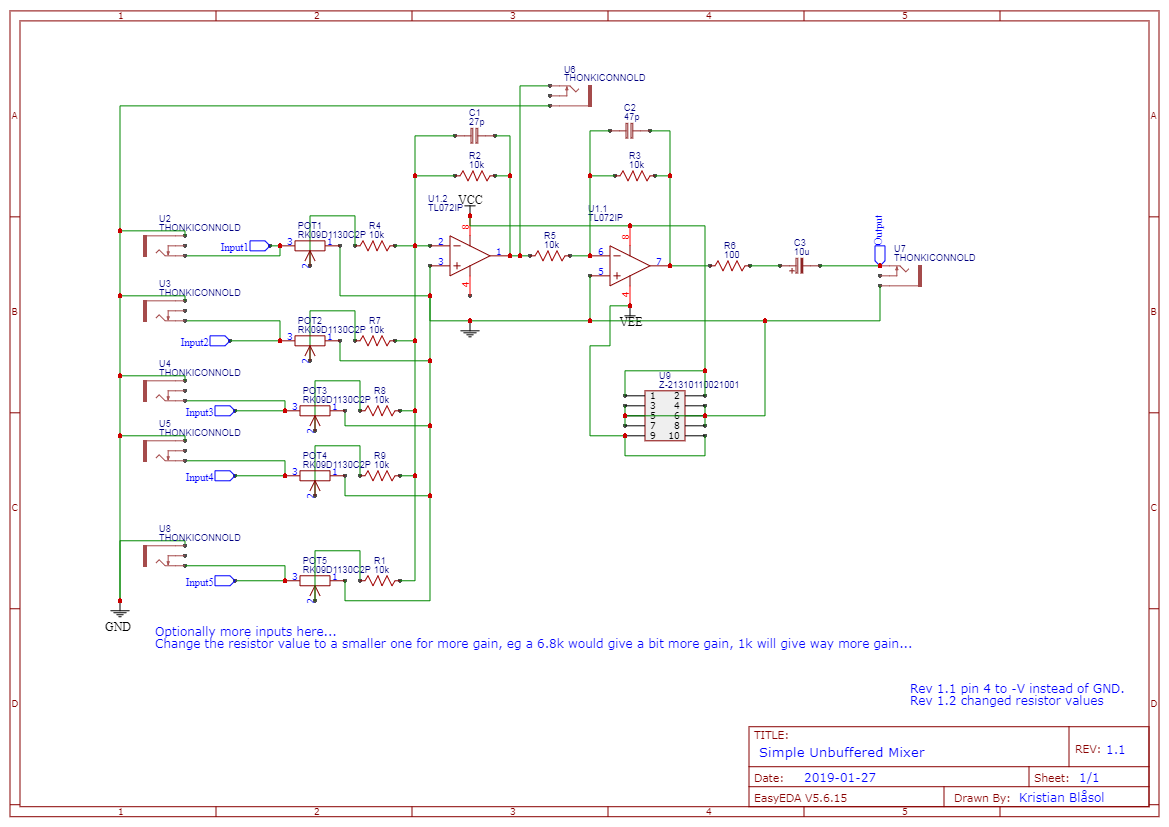
\includegraphics[width=.9\linewidth]{/home/felixp/Documents/diplomarbeit/dokumentation/figures/Schematic_Simple_Mixer.png}
\end{center}
\subsubsection{Benutzung}
\label{sec:orgb89eb20}
Die zu mixenden Signale werden durch die oberen drei Audiobuchsen angeschlossen. Die unterste Audiobuchse liefert das Ausgangssignal, wobei der rechtere der invertierende Ausgang ist. Als einfachen Patch könnte man die beiden Signale des \href{modules/oscillator.org}{Oszillator x2} Moduls zusammenführen um beide Oszillatoren auf einmal zu hören.

\subsection{Spannungskontrollierter Verstärker}
\label{sec:orga8db834}
Ein Spannungskontrollierter Verstärker (englisch: voltage controlled amplifier, oder VCA) verstärkt ein angelegtes Signal um einen Faktor, welcher proportional von einer \acl{CV} abhängt. \acp{VCA} sind essentiell, um den erzeugten Klängen einen Rhythmus zu verleihen, da ohne \ac{VCA} keine dynamische Lautstärkeänderung möglich ist. 
\subsubsection{Spezifikationen}
\label{sec:orgc5790de}
\subsubsection{Elektronik}
\label{sec:orgb9a2ca6}
Es gibt eine Vielzahl von möglichen Ansätzen für die technische Umsetzung eines \ac{VCA}. Die simpelste Möglichkeit ist es wohl, mit einer Vactrol zu verwenden, da diese mit nur minimaler Beschaltung zu einem VCA umgewandelt werden kann (schematic einfügen:\url{https://www.dropbox.com/s/o6oiyanco8lzmvt/Schematic\_Vactrol.pdf?dl=0}). Jede Art von \ac{VCA} hat einen gewissen Eigenklang wobei ein Vactrol-VCA eine sehr "`glatte"' Dynamik erzeugt. Abrupte Spannungsänderungen in der \acl{CV} werden geglättet, wodurch das ausgehende Signal nur eine stetige Änderung in der Lautstärke erfahren kann.

Ein weiterer Ansatz nutzt den linearen Reaktionsbereich zweier NPN-Transistoren, wobei durch die Beschaltung auf einem der Transistoren genau das gegenteilige Signal, allerdings mit dem gleichen positiven Offset erzeugt wird. Diese zwei Signale werden dann von einem Operationsvserstärker voneinander abgezogen, dadurch wird der positive Offset eliminiert und das modulierte Signal bleibt übrig. Es tragen eine Vielzahl von selbstregelnden Rückkopplungsschleifen dazu bei, dass diese Art von \ac{VCA} besonders stabil und schnell auf Änderungen in der Kontrollspannungen reagieren kann.
\subsubsection{Schematics}
\label{sec:org336516c}
\subsubsection{Benutzung}
\label{sec:org03a4a10}
\acp{VCA} können durch eine Vielzahl an Modulen angesteuert werden, am häufigsten ist wohl eine Art von Hüllkurvengenerator, um die Lautstärkeänderung bei einem Tastenanschlag zu simulieren. Ein einfacheres Beispiel wäre eine Rechteckswelle von einem LFO, um eine Art Stakkato zu erzeugen, oder ein langsam schwingender Sinus für eine Art Wobbel-Effekt.

\subsection{Attack-Release Hüllkurvengenerator}
\label{sec:org61cd6dd}
Hüllkurvengeneratoren sind Module, welche bei Eingang eines Gate-Signals eine Hüllkurve generieren. Diese kann beispielsweise dazu genutzt werden, um einen \ac{VCA} anzusteuern, um einem Klang Rhythmus und Dynamik zu verleihen. Aufgrund der Komplexität eines vollständigen \ac{ADSR} Hüllkurvengenerators haben wir uns dazu entschieden, einen simpleren \ac{AR} Hüllkurvengenerator zu bauen. Dieser besitzt einen Eingang für \acl{CV}, an welchen ein Gate-Signal angelegt werden kann und zwei Drehpotentiometer, durch welche die Parameter Attack und Release eingestellt werden können. Attack stellt dabei die Zeit dar, die das Signal nach dem Drücken einer Taste, beziehungsweise dem Anfang eines eingehenden Gate-Signals benötigt, um seinen Maximalwert zu erreichen. Release stellt die Zeit dar, die die Spannung der Hüllkurve nach dem Schließen des Gates benötigt, um wieder \SI{0}{\volt} zu erreichen.

\subsubsection{Spezifikationen}
\label{sec:org64febf8}
\subsubsection{Elektronik}
\label{sec:org60e1c3d}
In unserer Umsetzung wird das Potential am Eingang für \acl{CV}, an welchem ein Gate-Signal erwartet wird, von einem Operationsverstärkers auf 12V verstärkt. Durch den oberen Signalpfad füllt sich ein großer Kondensator, die Spannung, welche am Kondensator anliegt, wird gleichzeitig von einem Spannungsfolger gepuffert, da diese auch die Ausgangsspannung darstellt. Wird das Gate geschlossen, fällt die Spannung über den unteren Signalpfad wieder ab. Durch die Potentiometer kann man die Geschwindigkeit dieser beiden Prozesse kontrollieren.
\subsubsection{Schematics}
\label{sec:org69ad6a7}
\url{https://www.falstad.com/circuit/circuitjs.html?ctz=CQAgjCAMB0mRA2aYAcCDsLIE4BMBWSAZgxWxEIosgoFMBaMMAKAEMQAWLEXXDivDz4hyYXFHBwpNXMgQSw0yG0kcZa8GPU1R4moqVRYxIkTxowHXkUvoi+I3CK502G9nz2cuMvINTmACdObj4aLhpnGn0sOCCQ7QTNPRAUXADgjjB5dJRObJAohSV4-EFefgxxCol8BGVgpnSeDTECsOK4gBMQKvBBdHxxMHKQLtoAM1YAVwAbABdmHsHqut70VZyxyZmFpcKSHkg8rJzjnm2pucXg0zO8l2rz-RKAd2TEpsjIfmV3r8KP1U31+zH+Pxka0UGiIQOUAHN8vIiqdCkMJAikijuPYUpjsOgcig8gTkc1oswAMYiQlCfiknjEjHGOCoRzEFxuEaeQjmbDyGCssHrarCPoEAXC8Vijb9PTClZy1JwJV-ECKiXKyGS97mJV6mpqg3CA1rI0+Ok0nLCNWo3JJe3KABKSSaSQQvwkrTxRnwzBdHXtIyeeWinBoDjDMD9YHQ-FiSrQ-BqEH8Kpg6SIIAAgvN5qxKQBrZix+MqzVJxl5VOGGDYDxKRvwEBO2izWisADOtGFKGcluNoPeleDIgto7Vlc1pp1qX7PhJFoXUGFM7HDyZRtpKYhluUnZaMnOjyOofAIHmgWmPZI1dw7W9HsPGP96pQ-DEeXQQM-CnPkeZP1bytAdaVjAUVwAe0KdBek9AAPFBFDEI5wFkM9qhAegPBgwoqBoAB5aZ5gAB2mZggA}
\begin{figure}[htbp]
\centering
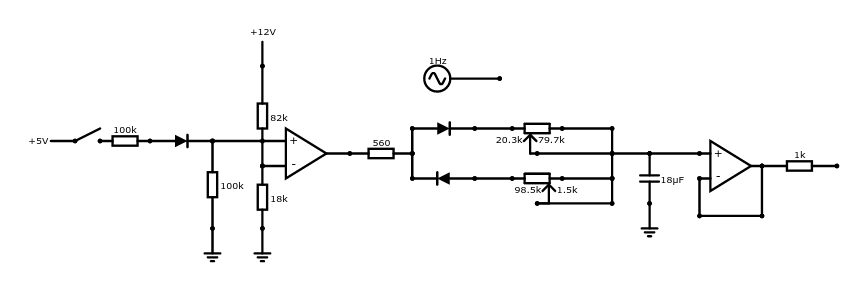
\includegraphics[width=.9\linewidth]{/home/felixp/Documents/diplomarbeit/dokumentation/figures/Schematic_AR.png}
\caption{Schaltkreis für einen simplen Attack Release Hüllkurvengenerator; Quelle: TODO}
\end{figure}
\subsubsection{Benutzung}
\label{sec:org426459b}
